\documentclass[10pt]{article}
\usepackage[top=2cm, bottom=2cm, left=2cm, right=2cm]{geometry}
\usepackage{graphicx}
\usepackage{multicol}
\usepackage[colorlinks=true]{hyperref}
\usepackage{verbatim}
\usepackage{enumerate}
\usepackage{wrapfig}

\title{Wesnoth UMC Development \\ Developer's Manual}
\author{Timotei Dolean - \href{mailto:timotei21@gmail.com}{timotei21@gmail.com}}

\begin{document}

\maketitle

\tableofcontents
\setcounter{tocdepth}{3}
\newpage

\newcounter{cnt}
\newcommand{\icnt}{ \stepcounter{cnt} \thecnt }

\section{Foreword}
\begin{multicols}{2}
 \begin{center}
    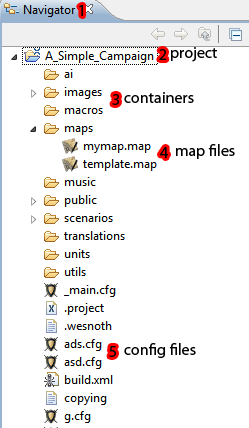
\includegraphics[scale=0.7]{definitions.png}
 \end{center}

The plugin's homepage is: \url{http://eclipse.wesnoth.org/} \\

Throughout this readme the following terms with the specified meaning will be used:
\begin{enumerate}
\item Navigator / Project Explorer / Package Explorer - an Eclipse view that shows the projects in the workspace
\item Project - a directory on the harddrive that is represented as a top directory in the navigator.
\item Container - this is a directory or a project. Basically it can contain any file or directory children.
\end{enumerate}

The image in the left highlights the terms used: 1 - Navigator, 2 - Project, 3 - Containers, 4 - Map files, 5 - Config files that contain WML code
\end{multicols}

\section{Prerequisites}
A quick list before getting into details:
\begin{enumerate}
\item Java 6 or 7 (8 won't work yet)
\item Python 2.x
\item Eclipse 3.7 (Indigo) or newer
\item Wesnoth 1.9.x, trunk or newer
\end{enumerate}

Now for getting all those items:
\begin{enumerate}
\item The plugin runs on the following platforms: Windows 32/64 bit, Linux 32/64 bit and Mac OS X 64bit. Note that \textbf{Mac OS X 32 bit} is \textbf{not supported}. If you want to know why, please consult the Frequently Asked Questions section.
\item Download and install Oracle's Java Version 7 (Java SE7): \href{http://www.oracle.com/technetwork/java/javase/downloads/jdk7-downloads-1880260.html}{Download JDK}

\textit{Note:} The plugin uses Java SE6/SE7, thus older versions (like 1.4 or 1.5) won't work with it.\\
\textit{Note:} Please double check the java installed on your system. On some machines there is the OpenJDK or other Java versions. Just use Oracle's so there will be no problems.

\item Download and install Python 2.x:
 \begin{enumerate}
   \item \textbf{Windows:} Download and install it from here: \href{http://python.org/download/}{Download Python} , selecting a 2.x version
   \item \textbf{Linux:} Use the distribution's package manager for installing it.
   \item \textbf{Mac:} Download and install it from here: \href{http://python.org/download/}{Download Python} , selecting a 2.x version
   \item For other operating systems, check the guide over here: \href{http://wiki.python.org/moin/BeginnersGuide/Download}{Python download and install}
  \end{enumerate}
 \textit{Note:} Please ensure you install the 2.x version. Version 3.x is \textbf{not} yet supported by the Wesnoth's WML Tools.

\item Download ``Eclipse" (The download links are in the right. Please ensure you are downloading at least the \textbf{3.7} version, otherwise the plugin will not work. Also, \textbf{don't} download a \textbf{64 bit version} unless you are sure you have Java JDK on 64 bit. If you are unsure, select the 32 bit version):  \href{http://eclipse.org/downloads/packages/eclipse-rcp-and-rap-developers/indigor}{Download Eclipse for RCP and RAP Developers}

\item Extract the downloaded archive in a known location and launch the executable (eclipse / eclipse.exe)

\item You will need to have a wesnoth version 1.9.x, trunk or newer, in order for the plugin's features to correctly work.
\end{enumerate}

\section{Setup the environment}
After you got all the prerequisites, you need to setup the eclipse installation.

\subsection{Target Platform setup}
\begin{enumerate}
\item Download the ``eclipse\_3.7.zip" archive, that contains an already existing Eclipse SDK installation and deltapack (used for building against other OSes than the native one). The link for the download is: \href{http://sourceforge.net/projects/wesnoth/files/wesnoth-umcplugin/build\_utils/eclipse\_3.7.zip/download}{Download}

\textit{Note:} You can generate the archive contents yourself by downloading the Eclipse SDK and its corresponding deltapack from \url{http://download.eclipse.org/eclipse/downloads/}.

\item Extract the archive somewhere.

\item Go to menu: Window -$>$ Preferences-$>$ Plug-in Development-$>$ Target Platform

\item Select the \textbf{Running Platform (Active)} item and press ``Edit..." in the left buttons lane.

\item A new window with tabs will be opened. Select the ``Locations" tab, and in the right buttons lane, select ``Add..."

\item Select ``Directory" in the new windows, then press Next.

\item Browse to the previous location where you have extracted the ``eclipse\_3.7.zip" archive.

\item Press Finish and OK until you exist all windows.
\end{enumerate}

\subsection{Installing Xtext}
\begin{enumerate}
\item Open up the ``Install new software" menu, and select from the list: ``Indigo - http://download.eclipse.org/releases/indigo" (if using a newer version, just select the url that starts with \emph{http://download.eclipse.org/releases})

\item In the list populated with items, select from the ``Modelling" category: ``Xtext SDK", and install it. Restart eclipse after that.

\item For the plugin's source, checkout the folder ``umc\_dev" from
  the Battle for Wesnoth repository.

\item In Eclipse, right click in \textbf{Package Explorer/Navigator} and then select \textbf{Import - General - Existing projects into Workspace}

\item Select the path where you downloaded the ``umc\_dev" folder, and check all the projects: ``org.wesnoth", ``org.wesnoth.dependencies.feature", ``org.wesnoth.feature", ``org.wesnoth.ui" and ``org.wesnoth.tests". \textbf{Don't} check the "Copy projects into workspace.

\item The projects will be compiled automatically. Just to be sure, as in each Java project, verify that the ``Build automatically" entry in the ``Project" menu is checked.
\end{enumerate}

\section{Running the plugin}
After you've setup the environment you can run the plugin.
\begin{enumerate}
	\item Go into the ``org.wesnoth" project.
	\item Select the ``plugin.xml" file, and double-click to open it.
	\item Click the ``Launch an Eclipse application" or ``Launch an Eclipse application in Debug mode" from the right part of the file, to launch the plugin.
\end{enumerate}
	\centerline{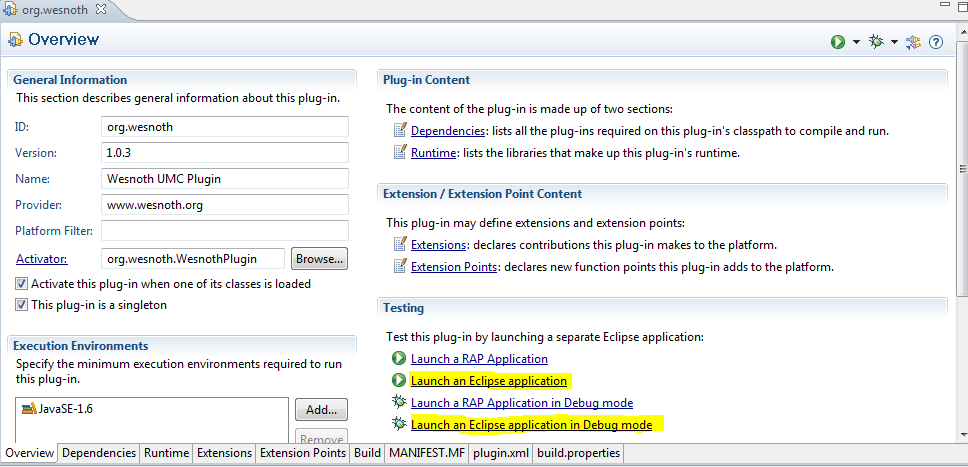
\includegraphics[scale=0.6]{launch_plugin.png}}

If you want to know how you can use the plugin, please consult the User's Manual.

\section{Running the tests}
\subsection{Normal tests}
The plugin has a Test Suite based on JUnit 4, that tests some aspects of plugin's working internals. A running instance of the plugin is not necessarily. To run these tests, follow the following steps:
\begin{enumerate}
	\item Go to the ``Run" menu, and select ``Run configurations..."
	\item In the left pane's list, right click on the ``JUnit" item
	\item Select ``New" from the opened context menu
	\item Select the first radio box: ``Run a single test"
	\item For the \textbf{Project}, enter: ``org.wesnoth.tests" ( or browse for it )
	\item For the \textbf{Test Class}, enter: ``org.wesnoth.tests.WMLTestsSuite" ( or ``Search..." for it. Just enter ``WMLTestsSuite" in the newly opened window, and select the item )
	\item For the \textbf{Test method}, let it as it is by default: ``(all methods)"
	\item In the ``Test runner" Combo Box select ``Junit 4"
	\item Go to the ``Arguments" tab, and in the ``VM Arguments" text box, enter: $-DwesnothWorkingDir=<path>$
	\item Replace the $<path>$ token with the current path to the wesnoth working directory ( it contains the data directory )
	\item Press ``Apply" and ``Run"
\end{enumerate}

\subsection{PDE Tests}
This tests involve starting the plugin, and launching the tests after it started. This is because some Eclipse's framework is used ( projects, etc ). To run these tests, follow the following steps:
\begin{enumerate}
	\item Go to the ``Run" menu, and select ``Run configurations..."
	\item In the left pane's list, right click on the ``JUnit Plug-in Test" item
	\item Select ``New" from the opened context menu
	\item Select the first radio box: ``Run a single test"
	\item For the \textbf{Project}, enter: ``org.wesnoth.tests" ( or browse for it )
	\item For the \textbf{Test Class}, enter: ``org.wesnoth.tests.WMLPDETestsSuite" ( or ``Search..." for it. Just enter ``WMLTestsSuite" in the newly opened window, and select the item )
	\item For the \textbf{Test method}, let it as it is by default: ``(all methods)"
	\item In the ``Test runner" Combo Box select ``Junit 4"
	\item Go to the ``Arguments" tab, and in the ``VM Arguments" text box, add the following arguments, separated by space: 
	\begin{enumerate}
		\item $-DisTesting=true$
		\item $-DwesnothWorkingDir=<path>$ ( Replace the $<path>$ token with the current path to the wesnoth working directory ( it contains the data directory ) )
		\item $-DwesnothExec=<path>$ ( Replace the $<path>$ token with the current path to the wesnoth executable )
		\item $-DwesnothWMLTools=<path>$ ( Replace the $<path>$ token with the current path to the wesnoth wml tools directory )
		\item $-DwesnothUserDir=<path>$ ( Replace the $<path>$ token with the current path to the user directory ( it contains the data/add-ons directory ) )
		\item $-DpythonPath=<path>$ ( Replace the $<path>$ token with the current path to the python binary ( for *nix systems, 'pyhon' will suffice ) )
	\end{enumerate}
	\item Press ``Apply" and ``Run"
\end{enumerate}	


\textit{Note:} You can always launch last run configuration with F11 - Debug / CTRL+F11 - Run. Alternatively, you can launch them by clicking near the green bug/run icon, on the little down arrow, and selecting the run configuration.

\section{Building the plugin}
The plugin can be built as a zip archive (usually) for different operating systems. The built application can be launched without any Eclipse prerequisites. This plugin's version is called \textbf{Standalone}. 

You now have 2 choices: Build the plugin from within Eclipse - this way you can build, say, just for your current OS/architecture - or you can use the already existing build script - that builds the plugin for all currently supported architectures.

\subsection{Building via Eclipse}
\begin{enumerate}
    \item Open Eclipse.
    \item Go into the ``org.wesnoth" project, and open the file ``org.wesnoth.product".
    \item In the bottom right part of the opened file, in section ``Exporting" there is a link: ``Eclipse Product export wizard". Click that.
    \item In the ``destination" group, select where you want the export/build to be done.
    \item Check the ``Generate metadata repository". You can also check ``Export for multiple platforms" if you want to build the plugin for other OSes/Architectures as well.
    \item Press Next if you have selected ``Export for multiple platforms" and select the desired OSes/Architectures.
    \item Finally press ``Finish" to do the building.
\end{enumerate}

\subsection{Building via the SCons build script}
\begin{enumerate}
    \item Go to the ``build" directory in the repository checkout.
    \item The build is done via Scons.
    \item When launching the build first time you need to specify the ``eclipsedir" argument that specifies the path to a valid Eclipse SDK + deltapack installation. The file you have previously downloaded (``eclipse\_3.7.zip") already contains this.
    \item You can invoke the build like: \textit{scons  eclipsedir=/path/to/eclipse-sdk-dir}. After the first run, the path is cached and you won't need to specify it anymore.
    \item The directory ``wesnoth\_umc\_dev" will contain now the built plugin as zip archives, while the ``update\_site" directory will contain the update site for the plugin.
\end{enumerate}

\section{Generating the WML Grammar}
The WML Editor uses the Xtext (\url{http://www.eclipse.org/Xtext/}) framework for getting the functionality an editor should have. The editor is based on the WML grammar defined in the ``org.wesnoth/src/org.wesnoth/WML.xtext" file.
The file is written in some EBNF variant (\url{http://www.eclipse.org/Xtext/documentation.html\#\#grammarLanguage})

To (re-)generate the wml grammar, right click the ``org.wesnoth/src/org.wesnoth/GenerateWML.mwe2", and select ``Run as" and after that ``MWE2 Workflow". If this is your first time running the MWE2 Workflow, you'll be prompted to download the ANTLR generator jar file. Press (y) and that will continue.

\section{Frequently Asked Questions}
\subsection{Where can I submit any bugs found?}
Go over to Wesnoth's bug tracker: \href{https://gna.org/bugs/?func=additem&group=wesnoth&bug_group_id=116}{Add new bug}. Please be as specific as possible. Also, if you have any logs, please attach them.

\subsection{Why Mac OS X 32 bit is not supported?}
Apple decided to manage itself the versions that can run on each Mac version. Thus the modern Java SE6 version - which is used by the plugin - is not available on 32 bit Macs but on 64 bit only. The 32 bit Macs have just Java SE5 version available. Trying to port the plugin to the ``outdated" Java version is not likely to be done, so please consider upgrading your OS.

\end{document}
